% ******************************* Thesis Appendix B ********************************

\chapter{Optimal Propulsive Landing}
\label{app2}
\ifpdf
\graphicspath{{Appendix2/}{Appendix2/}{Appendix2/}}
\else
\graphicspath{{Appendix2/}{Appendix2/}}
\fi


\section{Introduction}
In the absence of an atmosphere, landing a probe on the surface of a planet, moon or any other body can be achieved only through propulsive descent. These maneuvers involve significant periods of continuous thrusting where the thrust vector has to be steered significantly to achieve a soft landing.\\
There can be further constraints on the lander to be vertical to the ground by the end of the maneuver. These requirements have been addressed through optimal control theory to generate optimal trajectories for landing from orbit. DE has
been used to solve the optimal control problem. A strategy has been arrived at to select the minimum thrust level required to perform the optimal phase of the descent. An effective and robust methodology to handle high thrust propulsive landing problems from orbit has been established in this study using differential
evolution. Both time optimal and fuel optimal formulations can be used to obtain solutions. The state and costate dynamics along with the optimal control law remain unchanged even though this is a high thrust problem. For demonstration, propulsive landing on Jupiter's moon Callisto has been considered.
\section{Results}
\subsection{Sample optimal landing trajectory}
The problem considered here is landing a 1500kg initial mass spacecraft with a thrust of 2000N and $I_{sp}$ of 315s. The current results are presented for the time optimal formulation.\\
The initial orbit around Callisto is a 100x100km circular orbit. The terminal conditions are set as achieving an altitude $50m$ above the surface of Callisto with a downward velocity of only $0.75m/s$. The horizontal component of velocity is set to be zero. This $50m$ altitude is considered as the target altitude as there needs to be a closed loop guidance procedure for the touch down phase as the surface topology may affect landing site location. This target altitude is also useful for sky-crane type of landing strategies which requires the lander to switch over from an optimal mode to a closed loop touchdown mode.\\
\begin{figure}[ht!]
	\centering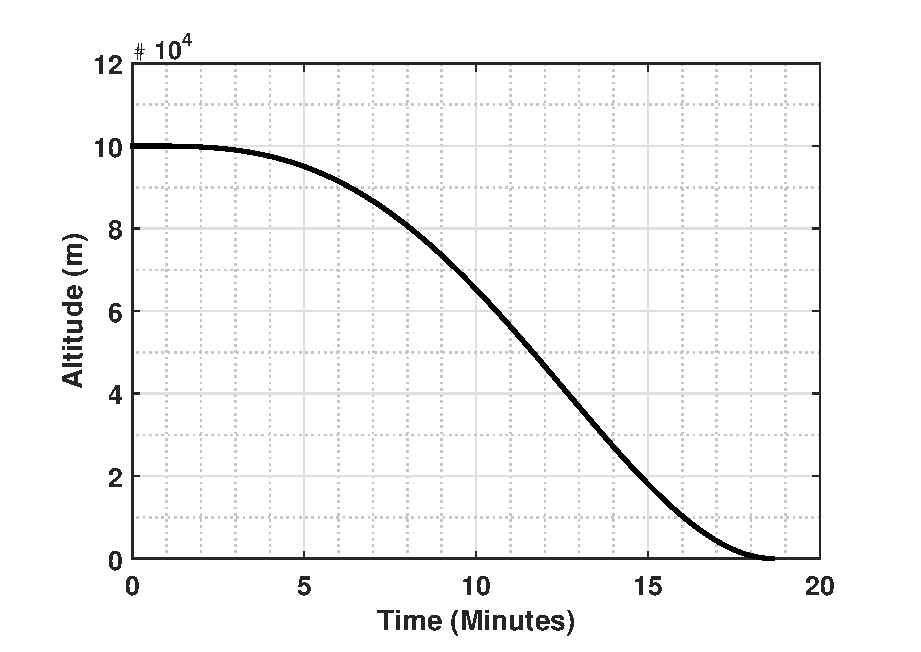
\includegraphics[width=0.90\linewidth]{Altitude.eps}
	\caption{Altitude profile for time optimal descent.}
	\label{altitude}
\end{figure}
During descent as seen in figure \ref{altitude}, the altitude of the spacecraft increases by a few meters initially. This increasing trend has been observed before in literature \citep{ramanan2005analysis}. This happens in the retrograde thrust phase where a significant fraction of the spacecraft's orbital velocity is negated. Due to the imposition of the optimal control law, a slight thrust angle exists off the tangential retrograde direction. This is the cause for the orbit raising. The next phase comprises of a rapid descent as the trajectory the spacecraft is elliptic with respect to Callisto. The final stage of the optimal trajectory involves a gradual drop in the altitude to the target value. This is essential for propulsive descent with a soft landing.\\
\begin{figure}[H]
	\centering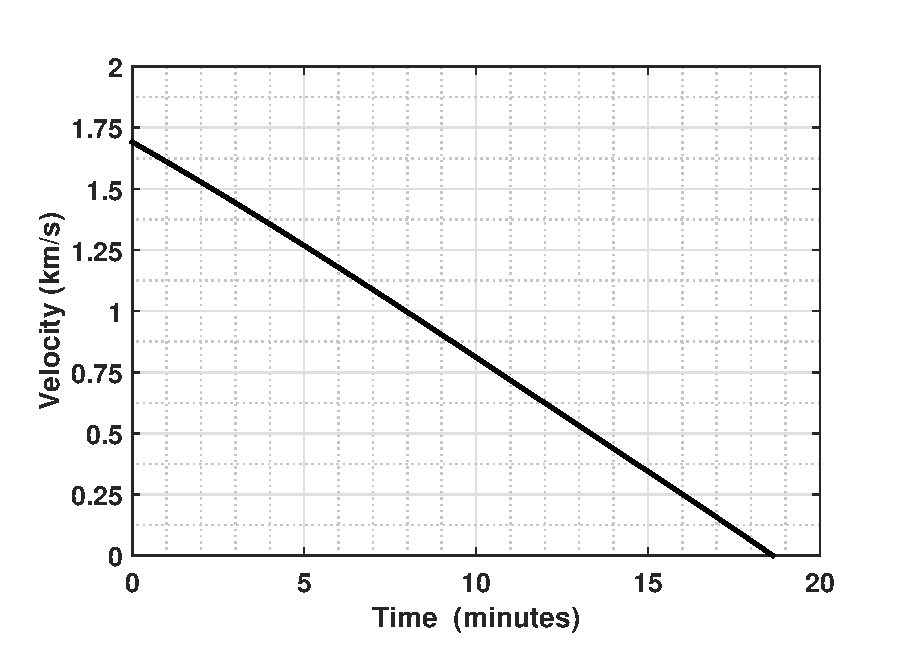
\includegraphics[width=0.90\linewidth]{Speed.eps}
	\caption{Velocity profile for time optimal descent.}
	\label{speed}
\end{figure}
\begin{figure}[H]
	\centering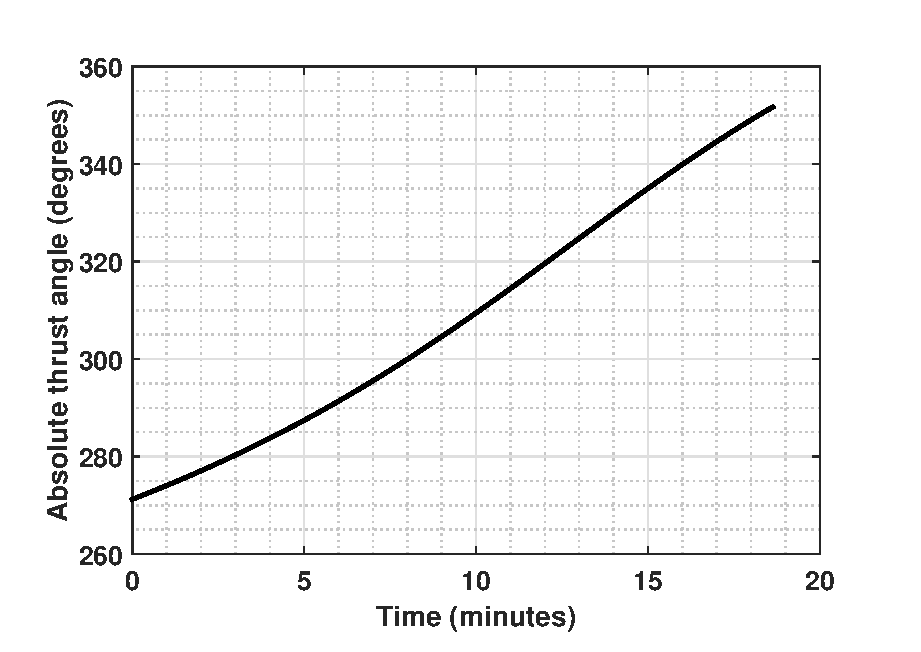
\includegraphics[width=0.9\linewidth]{Angle.eps}
	\caption{Thrust angle profile for time optimal descent.}
	\label{angle}
\end{figure}
In figure \ref{speed}, it is seen that the velocity of the spacecraft drops nearly linearly. The terminal deceleration at the end of the optimal phase is quite high as the thrusters are not throttled down. This leads to the requirement of imposing either acceleration limits in the optimal control formulation or by handling the terminal descent through a separate closed loop control. The latter strategy will be safer as it allows for the handling of landing obstacles in real time. In figure \ref{angle}, the thrust angle shows the steering requirement for the thruster. About $80^o$ worth of steering has to be performed by the attitude control thrusters. This is a small requirement and the steering rate is also quite low with a maximum of about $0.0863$ degrees per second. This can be managed by small attitude control thrusters. It is concluded that the optimal control profile generated by a 3DOF code for landing does not impose any severe attitude control requirements.
\begin{figure}[H]
	\centering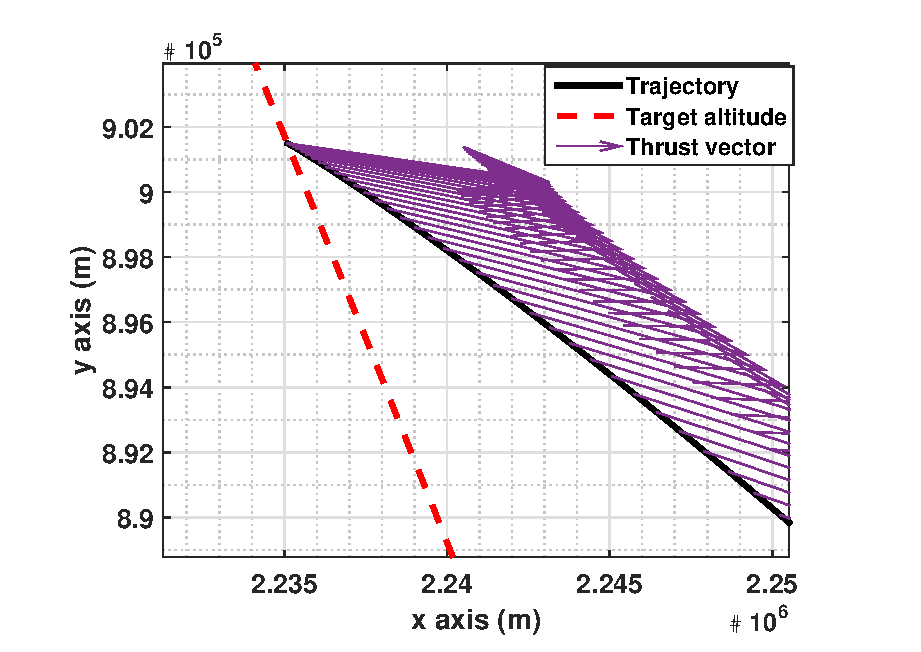
\includegraphics[width=0.9\linewidth]{Traj_end.eps}
	\caption{Final phase of optimal descent trajectory.}
	\label{traj_end}
\end{figure}
Fig. \ref{traj_end} depicts the final trajectory phase of the lander as it approaches the target altitude 50m above the surface of Callisto. Due to the high acceleration, only at the final instant of time, is the target velocity achieved. Even though in the plot, it seems to appear that there is a significant horizontal component, it is actually reduced to zero only at the final time. This is yet another reason for the optimal phase to end at $50m$ above the surface. The high thrust levels involved in the optimal descent phase can lead to excessive control requirements if continued till touchdown. Once the optimal phase causes the lander to attain the fixed target altitude, the lander has to switch over to closed loop guidance and control for landing at much lower acceleration levels. Even though the subsequent strategy is sub-optimal, it leads to a much better controlled landing and lower impact loads. The final velocity is made vertical to the Callisto's surface with a value of $0.75m/s$. Due to low velocity and high acceleration, this vertical velocity is achieved even though the approach of the lander prior to the terminal phase is significantly away from the vertical. This is made possible by the thrust steering law provided by the optimal control formulation.\\
\begin{figure}[H]
	\centering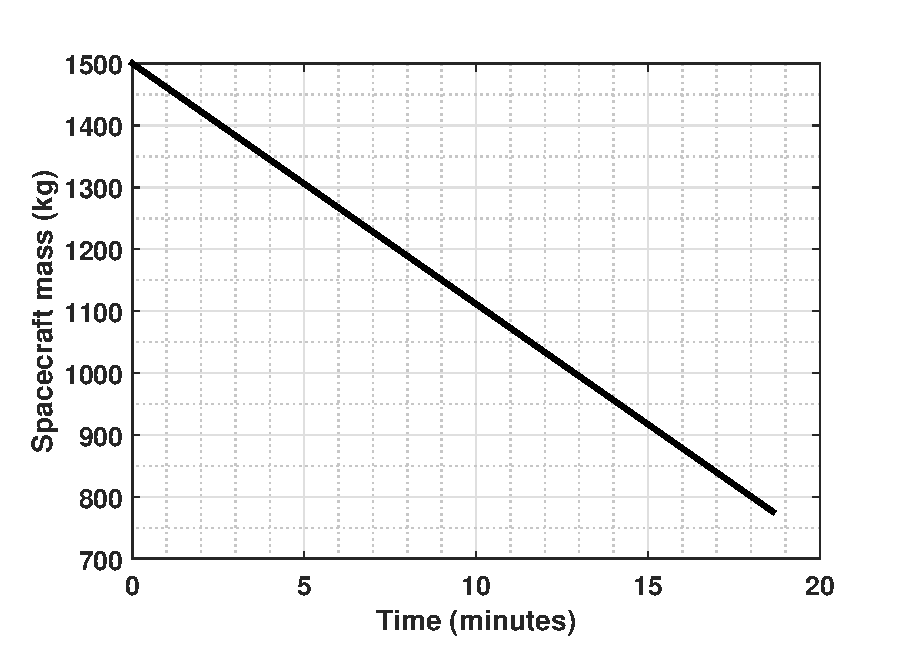
\includegraphics[width=0.90\linewidth]{Mass.eps}
	\caption{Spacecraft mass variation during descent.}
	\label{mass:fig}
\end{figure}

Figure \ref{mass:fig} shows the variation of the spacecraft's mass during the descent. This is exactly linear as the thrust is constant without any throttle. Due to this, the thrust acceleration on the spacecraft varies from $1.333m/s^2$ to $2.577m/s^2$ with the magnitude linearly increasing with time. The maximum deceleration that the spacecraft experiences is still lesser than any launch loads and is thus safe.

\subsection{Parametric studies: Time optimal results}
Figures \ref{fig:parametric:1} and \ref{fig:parametric:2} present the results of a parametric study on the fuel fraction and peak altitude to initial altitude ratio as a function of the initial acceleration level.
\begin{figure}[H]
	\centering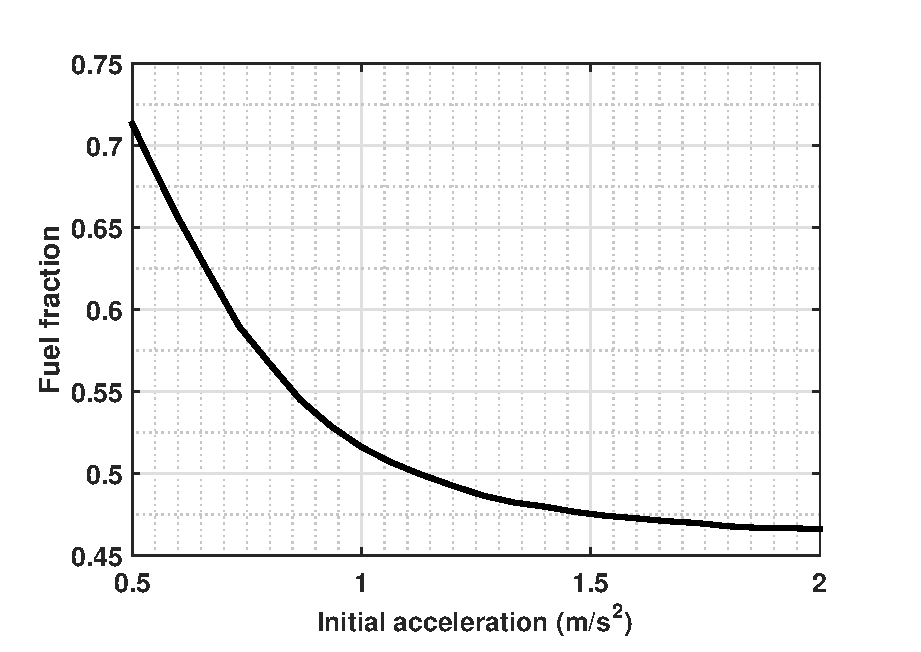
\includegraphics[width=0.90\linewidth]{fuelvsaccl.eps}
	\caption{Influence of initial acceleration levels on fuel fraction.\label{fig:parametric:1}}
\end{figure}
\begin{figure}[H]
	\centering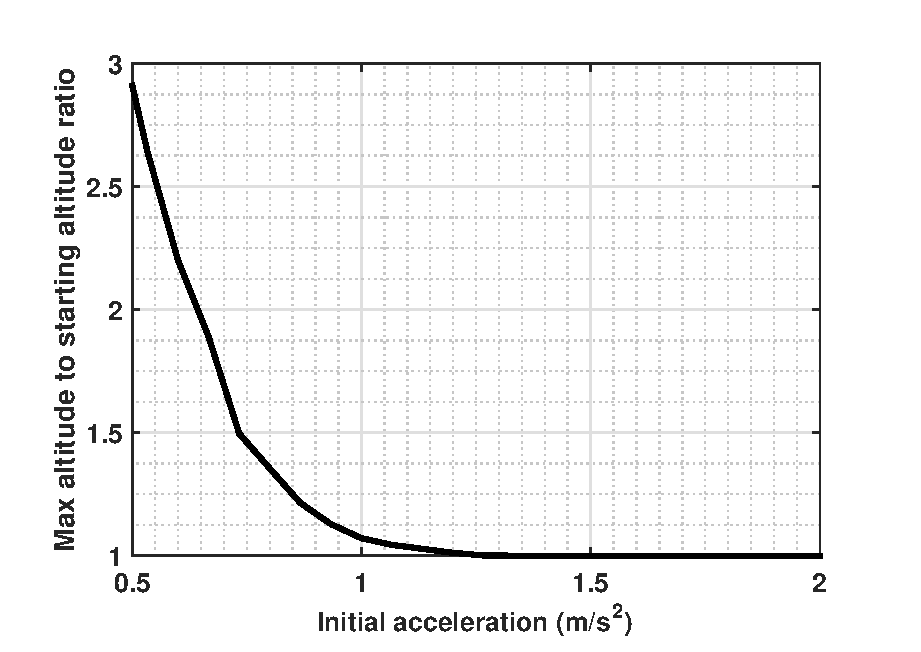
\includegraphics[width=0.90\linewidth]{altvsaccl.eps}
	\caption{Influence of initial acceleration levels on the peak to initial altitude ratios.\label{fig:parametric:2}}
\end{figure}
The transfer geometry and thruster specific impulse are taken to be the same as in the previous problem. It is clear that for very low initial accelerations, the fuel fraction is considerably higher due to the peak altitude climbing above the initial level. This is done to bleed off some mass so that the spacecraft gets lighter in order for the propulsion system to be able to handle the spacecraft in the presence of the central body's gravity. The fuel fraction drops asymptotically to about $0.466$ for this problem. Beyond a certain threshold thrust level, the trajectory only follows a downward path as the thrusters are now powerful enough to handle the entire spacecraft without having to bleed off extra mass. This study can be used to determine a suitable thruster configuration for a lander based on the fuel margins available and fix the minimum thrust level that would satisfy the weight constraints on the lander. These parametric studies have been done for the same initial and final orbits as the previous case.
\subsection{Parametric studies: Influence of specific impulse}
For this purpose, the same initial conditions are chosen but the final target altitude is set as 2km with the target velocity left free. The specific impulse is also varied by $\pm 5s$ from the nominal expected value. The propellant mass required by a 1500kg lander is depicted in figure \ref{fig:parametric:3}.
\begin{figure}[H]
	\centering\includegraphics[width=0.90\linewidth]{FuelvsTerminalSpeed.eps}
	\caption{Propellant required vs final velocity of optimal phase.}
	\label{fig:parametric:3}
\end{figure}
This type of parametric study helps in determining reserve propellant volumes needed based on the control requirements and variations in the engine's specific impulse due to environmental and manufacturing effects. 
\subsection{Parametric studies: Fuel optimal results}
Here the problem of landing an 874kg spacecraft with a 2200N thruster from a $100km\times 15km$ orbit around Earth's moon is considered with a target altitude of $0m$ and a target velocity of $0m/s$.
\begin{figure}[H]
	\centering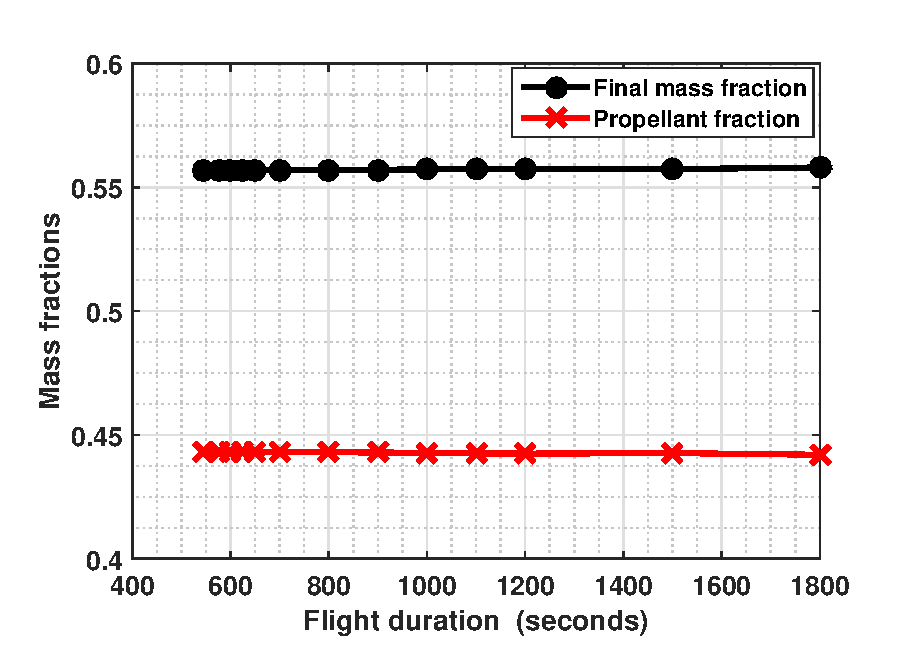
\includegraphics[width=0.90\linewidth]{FuelOpt_massfracs.eps}
	\caption{Influence of the flight duration on the fuel fraction and final delivered mass.}
	\label{fig:parametric:4}
\end{figure}
In figure \ref{fig:parametric:4}, it is seen that increasing flight duration causes a small drop in the fuel fraction with the final mass fraction delivered rising by a corresponding amount. This rise is only of the order of 0.8kg for over a $200\%$ rise in flight duration. Flight durations less than the time optimal value are not feasible solutions. This implies that unlike in the case of interplanetary transfers, increasing flight duration for  optimal propulsive landing does not lead to significant savings in propellant mass. The increase in flight duration is managed by the generation of coast phases by the optimal control formulation. These type of trajectories with higher flight duration can be useful if there are constraints on the communication requirements as well as on the navigation, guidance and control systems. The increased flight duration can serve to allow for corrections or system resets in case of emergencies.
\begin{figure}[H]
	\centering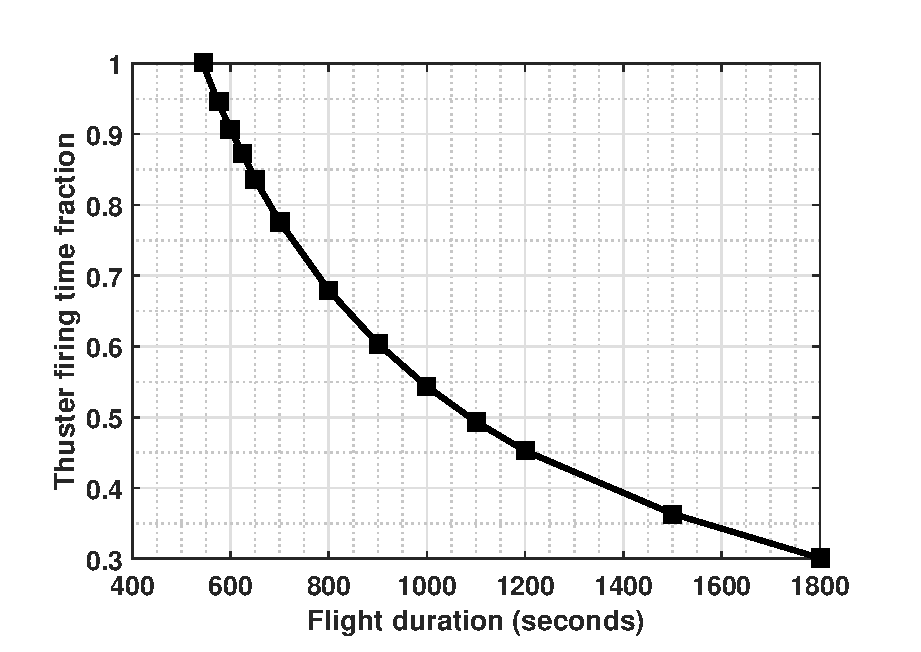
\includegraphics[width=0.90\linewidth]{ThrusterOnTime.eps}
	\caption{Fraction of time thruster is firing with varying flight duration.}
	\label{fig:parametric:5}
\end{figure}
Figure \ref{fig:parametric:5} shows results for the fraction of time the thruster is firing versus the total flight duration. In the time optimal formulation, it is seen that the thruster is continuously firing throughout. For increased flight duration, the thruster firing time fraction rapidly drops due to the appearance of a coast phase in the control leading to a thrust-coast-thrust control structure. This fraction varies such that the total thruster firing time is nearly a constant as the propellant consumption varies only by about $0.21\%$.
\section{Conclusions}
DE has been successfully applied to solve the problem of optimal propulsive descent. The results for landing a probe on Callisto have been presented along with a parametric study on the influence of the initial acceleration levels. Differential evolution has been shown to work for time optimal propulsive descent trajectories for a wide range of inputs. It has been hypothesized that selecting the minimum acceleration level which prevents the trajectory from rising to a value higher than the initial level will lead to an appropriate compromise between thrust level required and fuel fraction needed to perform the landing. The validity of this can be either proved or disproved by conducting several more parametric studies on the influence of initial acceleration to the fuel fraction and altitude ratio. The author is of the opinion that the proposed design strategy is suitable for realistic optimal lunar lander trajectory design. Fuel optimal parametric results have been generated and it has been demonstrated that it is possible to have large increases in flight duration to satisfy other mission requirements without any compromise on the fuel fraction required.
This is a demonstration of the capability of the current formulation to handle high thrust trajectory design cases. Several important trends in the results have been documented. A strategy is proposed to select the minimum thrust level required based on optimal control results. Fuel optimal soft landing trajectories have been generated and the capability of the formulation to handle large coast durations even in the high thrust case has been shown.\\